\documentclass[letterpaper,11pt]{report}

\usepackage[T1]{fontenc}
\usepackage[spanish]{babel}
\usepackage{hyphsubst}
\usepackage[utf8]{inputenc}
\usepackage{graphicx}
\graphicspath{ {./img/} }
\usepackage{color}
\usepackage{xcolor}
\usepackage{url}
\usepackage{textcomp}
\usepackage{listings}
\usepackage{parskip}
\usepackage{lettrine}
\usepackage{newcent}
\usepackage{setspace}



\begin{document}

\pdfinfo{
   /Author (Ronaldo Gligan)
   /Title  (El salmonete Roger y su miserable vida)
}

\begin{center}
%\vspace*{\fill}
%\thispagestyle{empty}
\pagenumbering{gobble}
{\Large El salmonete Roger y su miserable vida}\\*[0.4in]
Ronaldo Gligan\\*[0.2in]
\textit{Ilustraciones de} \\ Alim Martínez Botashev\\*[0.2in]

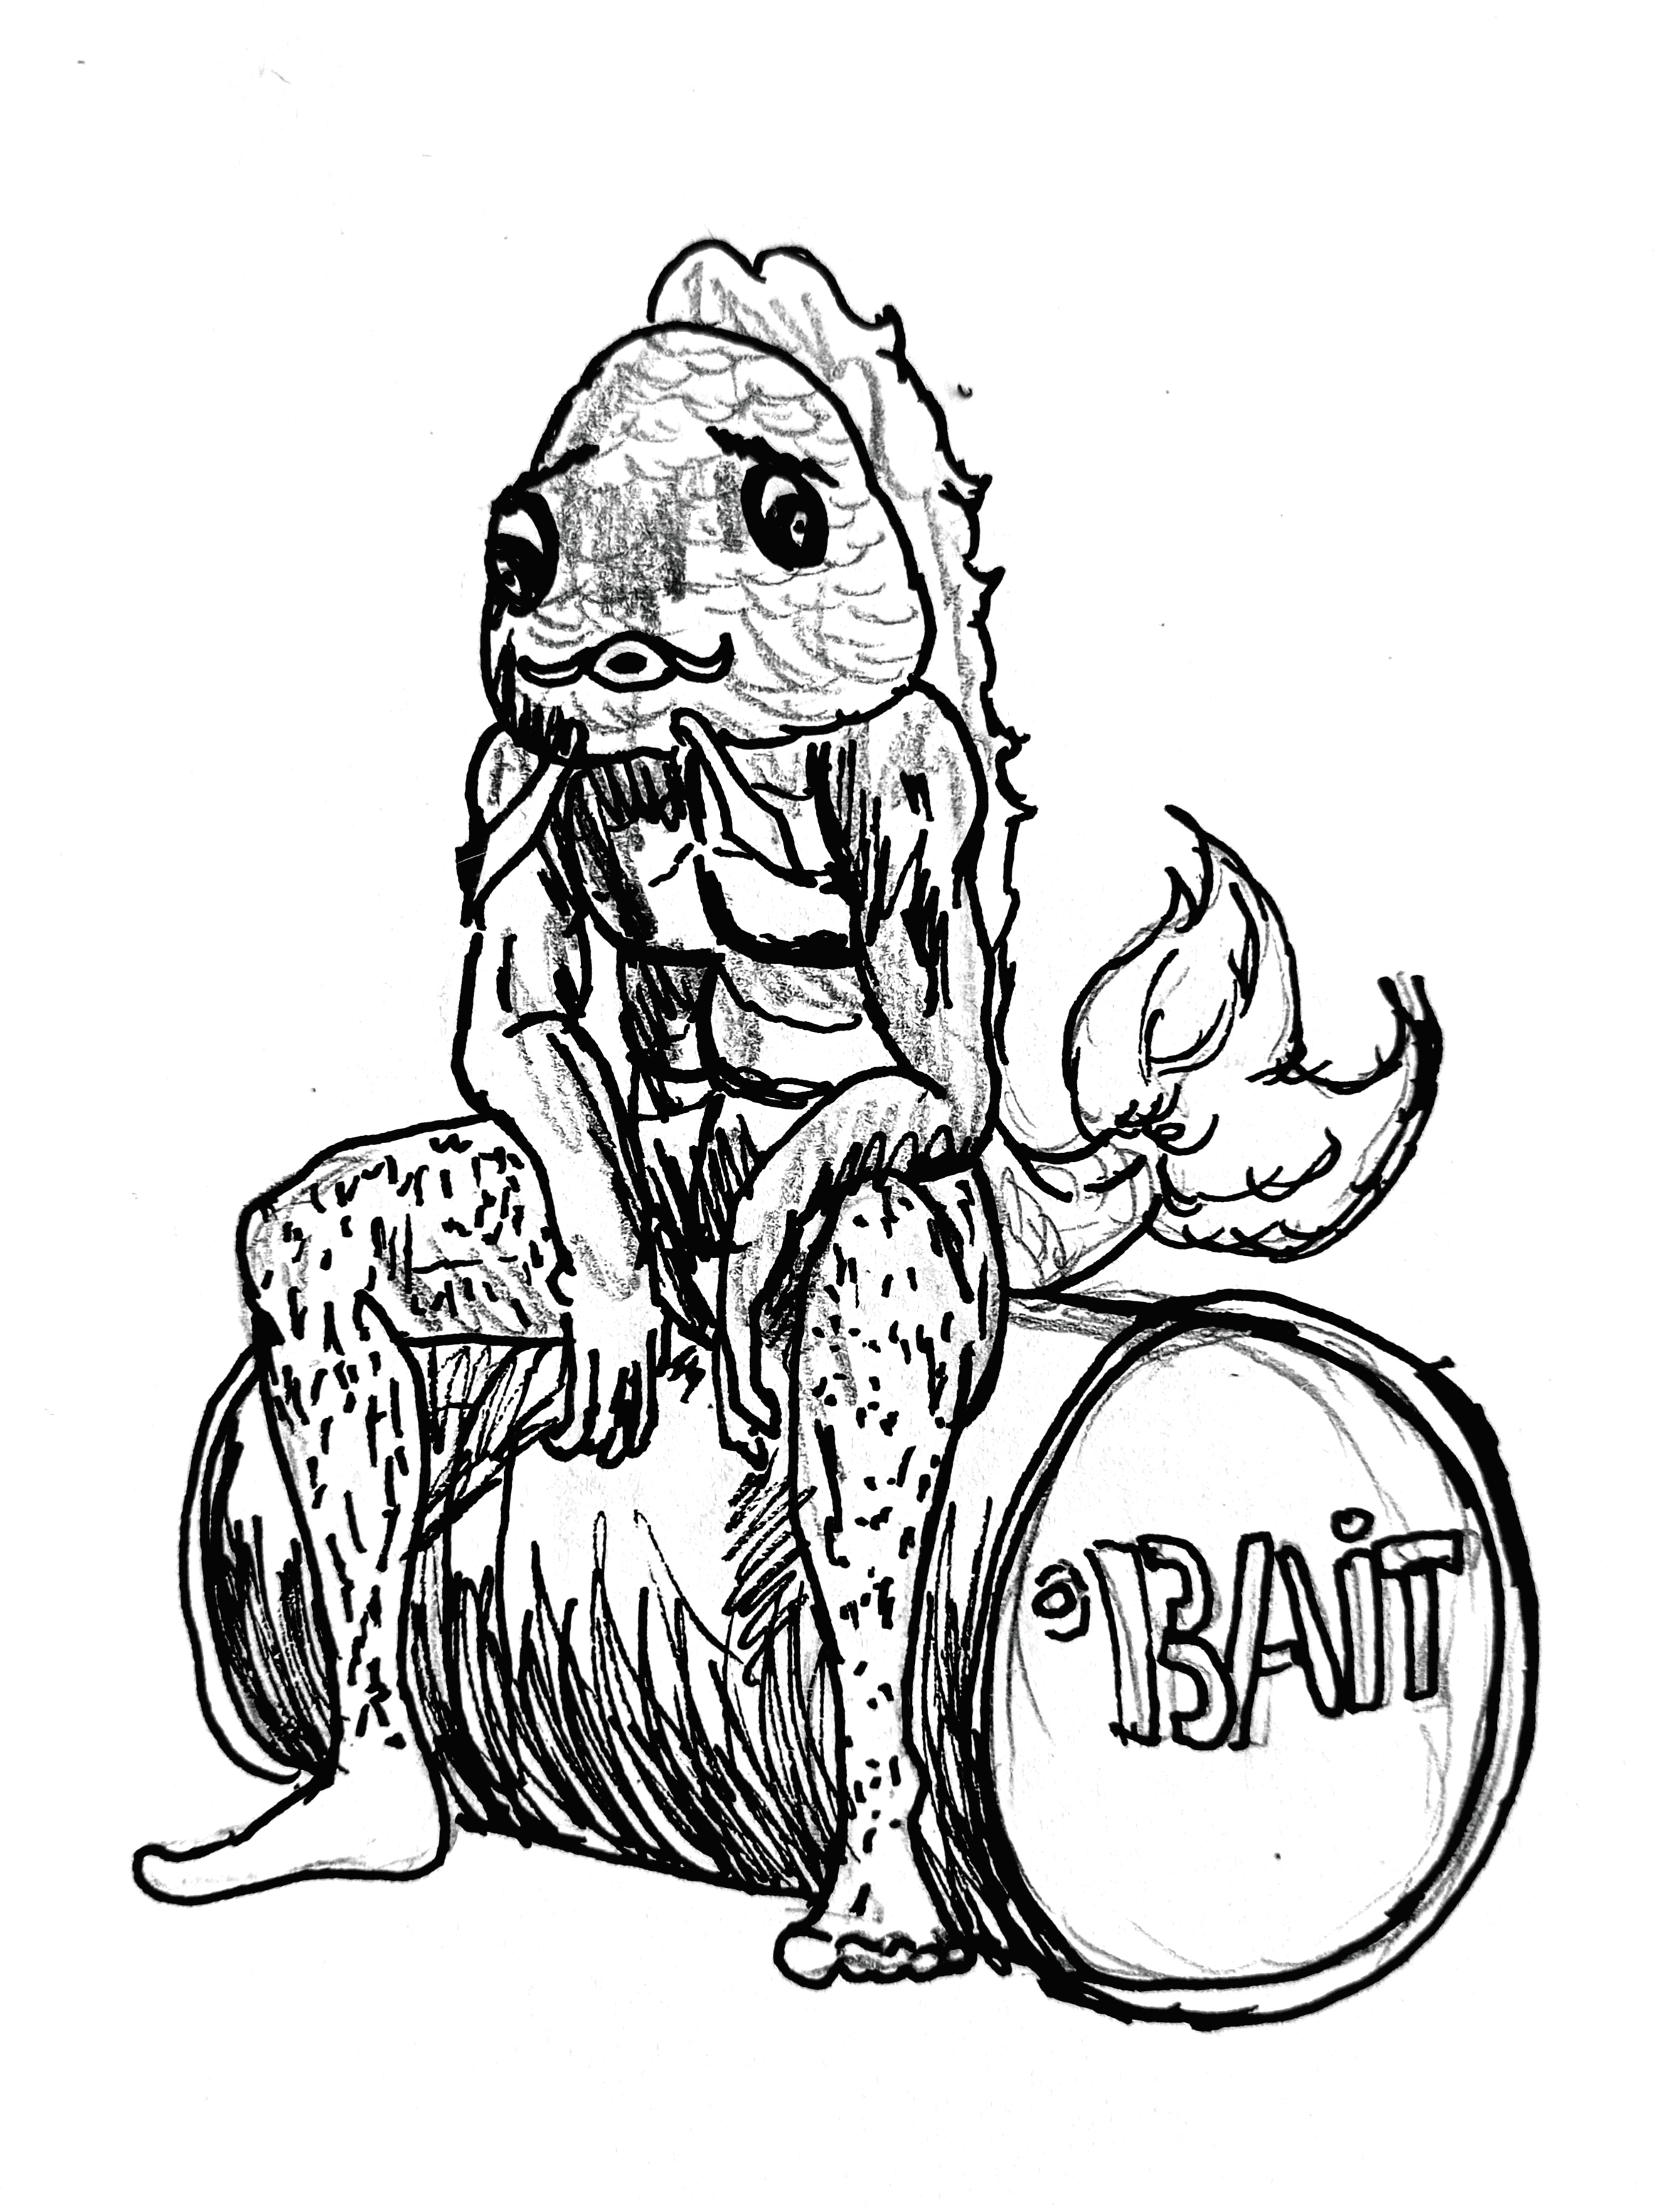
\includegraphics[scale=0.13]{1}

%\vspace*{\fill}
\pagebreak
\end{center}


\topskip0pt
\vspace*{\fill}

\begin{quote}\begin{quote}\begin{quote}%\begin{quote}
\begin{flushleft}
    \setstretch{1.4}
    \textit{Agradezco incondicionalmente a los alumnos y profesores de} 1º \textsc{bah} \textit{del curso} 2021--2022 \textit{del} \textsc{ies} Libertas. \textit{Sinceramente, sin ellos, esta obra no hubiese existido.}
\end{flushleft}
\end{quote}\end{quote}\end{quote}%\end{quote}

\vspace*{\fill}
\pagebreak

%\chapter*{}
\pagenumbering{arabic}

%\vspace*{\fill}

\begin{center}
\begin{tabular}{l}
\textit{Un simple pez}\\
\textit{Un pez que nada}\\
\textit{Y que Carles ama}\\
\\
\textit{Un salmonete}\\
\textit{Un pez que nada}\\
\textit{Y que todos quieren}\\
\\
\textit{Este pez es especial}\\
\textit{Un pez que nada}\\
\textit{Y que a todos gusta}\\
\\
\textit{Roger, el salmonete}
\end{tabular}
\end{center}

\vspace*{\fill}

\lettrine{E}{n} una mañana de abril el salmonete Roger salió de su lúgubre cueva y miró a su alrededor. Tenía que volver a empezar otra vez. No podía más. Tres años habían pasado desde que la última vez que vio la luz del sol. Tres años desde que la última vez que comió una comida decente. Tres años desde que la última vez que tuvo una conversación inteligente. Tres años desde que la última vez que sintió la felicidad.

Roger era un salmonete, un pez que habitaba en los ríos de Europa. Y en estos ríos, los salmonetes tenían una vida difícil. Debían nadar constantemente contra la corriente para llegar a los lugares donde podían desovar. Y luego, una vez que hubieran puesto sus huevos, tenían que volver a nadar contra la corriente hasta llegar a los ríos donde podían vivir.

Pero a Roger no le importaba nadar contra la corriente. De hecho, le gustaba. Le gustaba el desafío de luchar contra las fuerzas de la naturaleza. Y le gustaba la sensación de logro que experimentaba cuando finalmente lograba llegar a su destino.

Pero hacía tres años, todo había cambiado para Roger. En ese entonces, estaba nadando en un río francés cuando fue atrapado por un pescador. Roger fue arrastrado hasta la orilla. Esta vez no podía nadar contracorriente. Luego, el pescador lo sacudió fuera de su anzuelo y lo arrojó a un barril lleno de agua. Roger no podía creer lo que le estaba pasando. Nunca había sido atrapado antes y no sabía qué hacer.

\begin{center}
    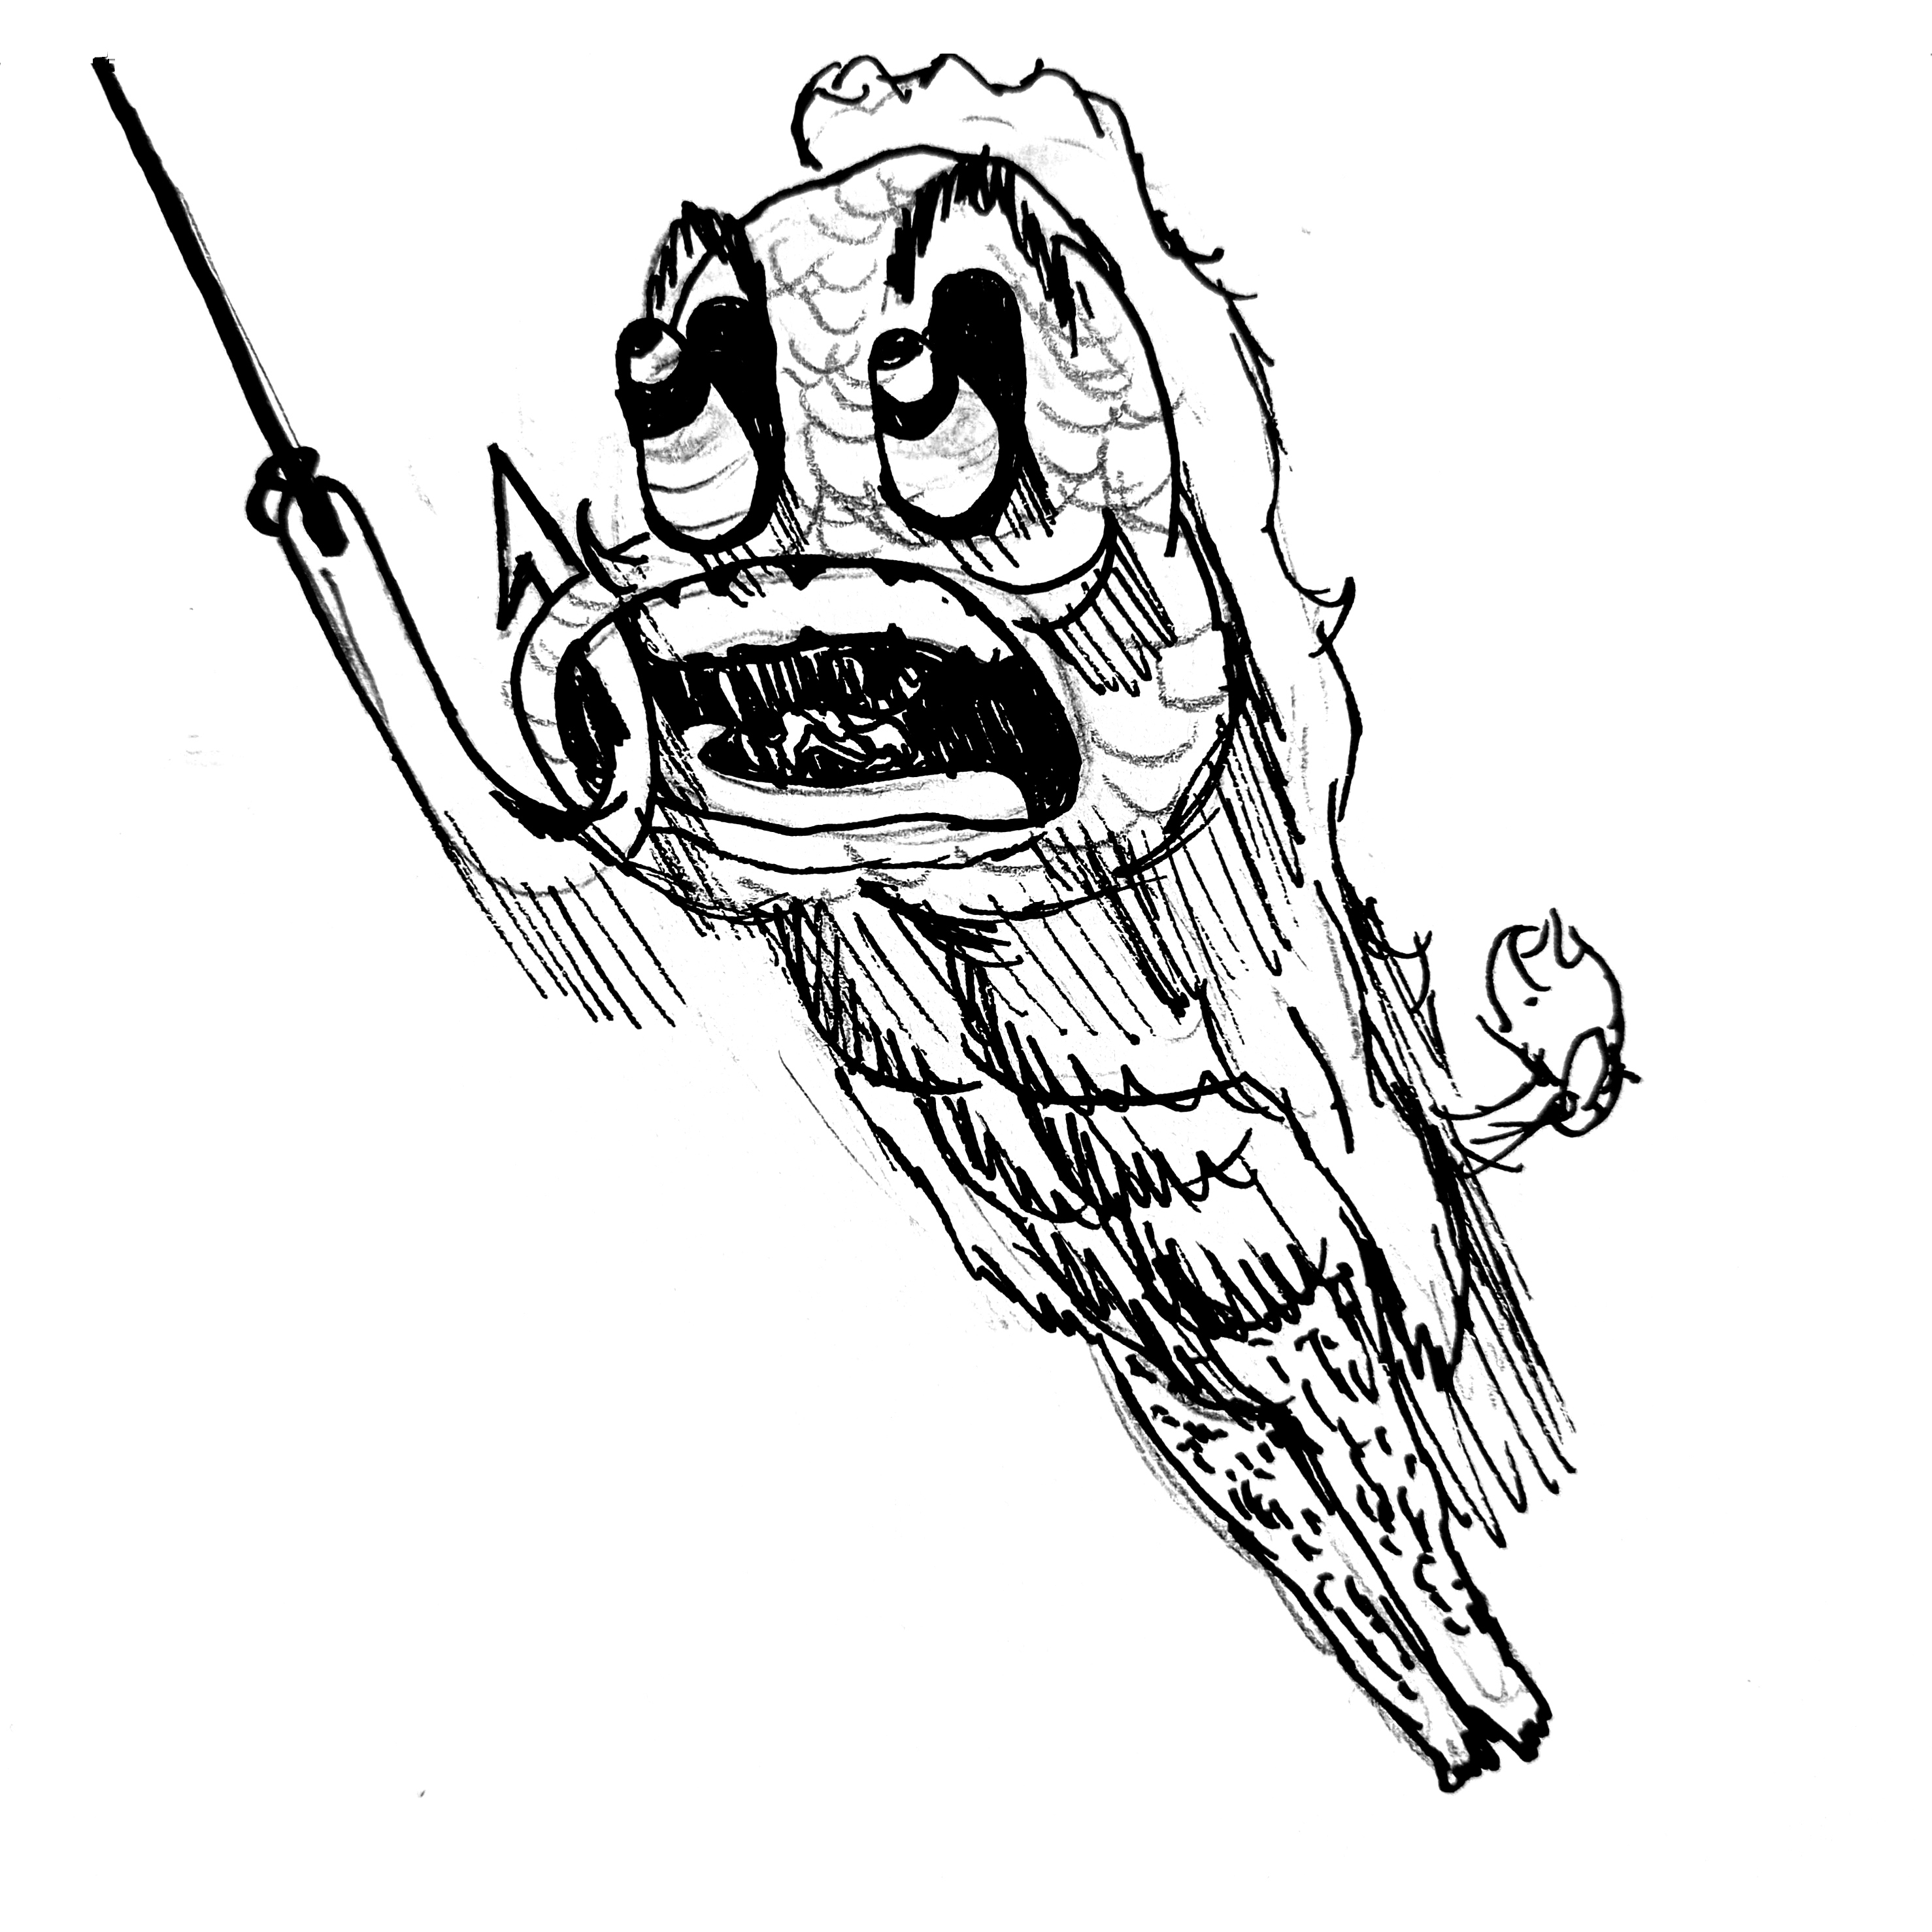
\includegraphics[width=0.5\textwidth]{2}
\end{center}

En el barril, Roger no podía nadar contra la corriente. No podía moverse libremente. Y el agua en el barril se estaba volviendo cada vez más sucia. Roger estaba asustado y solo. No sabía cuánto tiempo iba a estar en el barril, pero sabía que no era un lugar para un pez como él. El barril fue abierto y Roger fue sacado del agua. Fue arrojado a una caja de cartón y luego metido en un camión. Roger se asfixiaba. Necesitaba su hálito vital; su agua. El camión se puso en marcha y Roger supo que su vida estaba a punto de cambiar para siempre.

En el camión habían otros peces, salmonetes como él. Le contaron a donde iban: el “acuario” del “zoológico”. Roger no sabía qué eran esas palabras, pero supo que no sonaban bien. Cuando llegaron al “acuario”, Roger fue metido en una pequeña jaula de acero. Estaba isolado. La jaula era muy parecida a su cueva, pero Roger no se sentía como en casa. No había corrientes de agua para nadar contra y el agua en la jaula estaba estancada y sucia. Roger no podía creer que este fuera el lugar en el que iba a pasar el resto de su vida.

Roger pasó los primeros días de su cautiverio tratando de escapar de la jaula. Luchaba contra las paredes de acero, pero era inútil. No podía salir. Después de un tiempo, Roger se dio por vencido y se dejó caer en el fondo de la jaula. No quería comer, no quería nadar, no quería hacer nada. Se sentía miserable y solo. No sabía cómo iba a sobrevivir en este lugar.

Un día, cuando Roger había perdido toda la esperanza, se le acercó un niño. Le preguntó cómo se llamaba. “Soy Roger,” dijo.

\begin{center}
    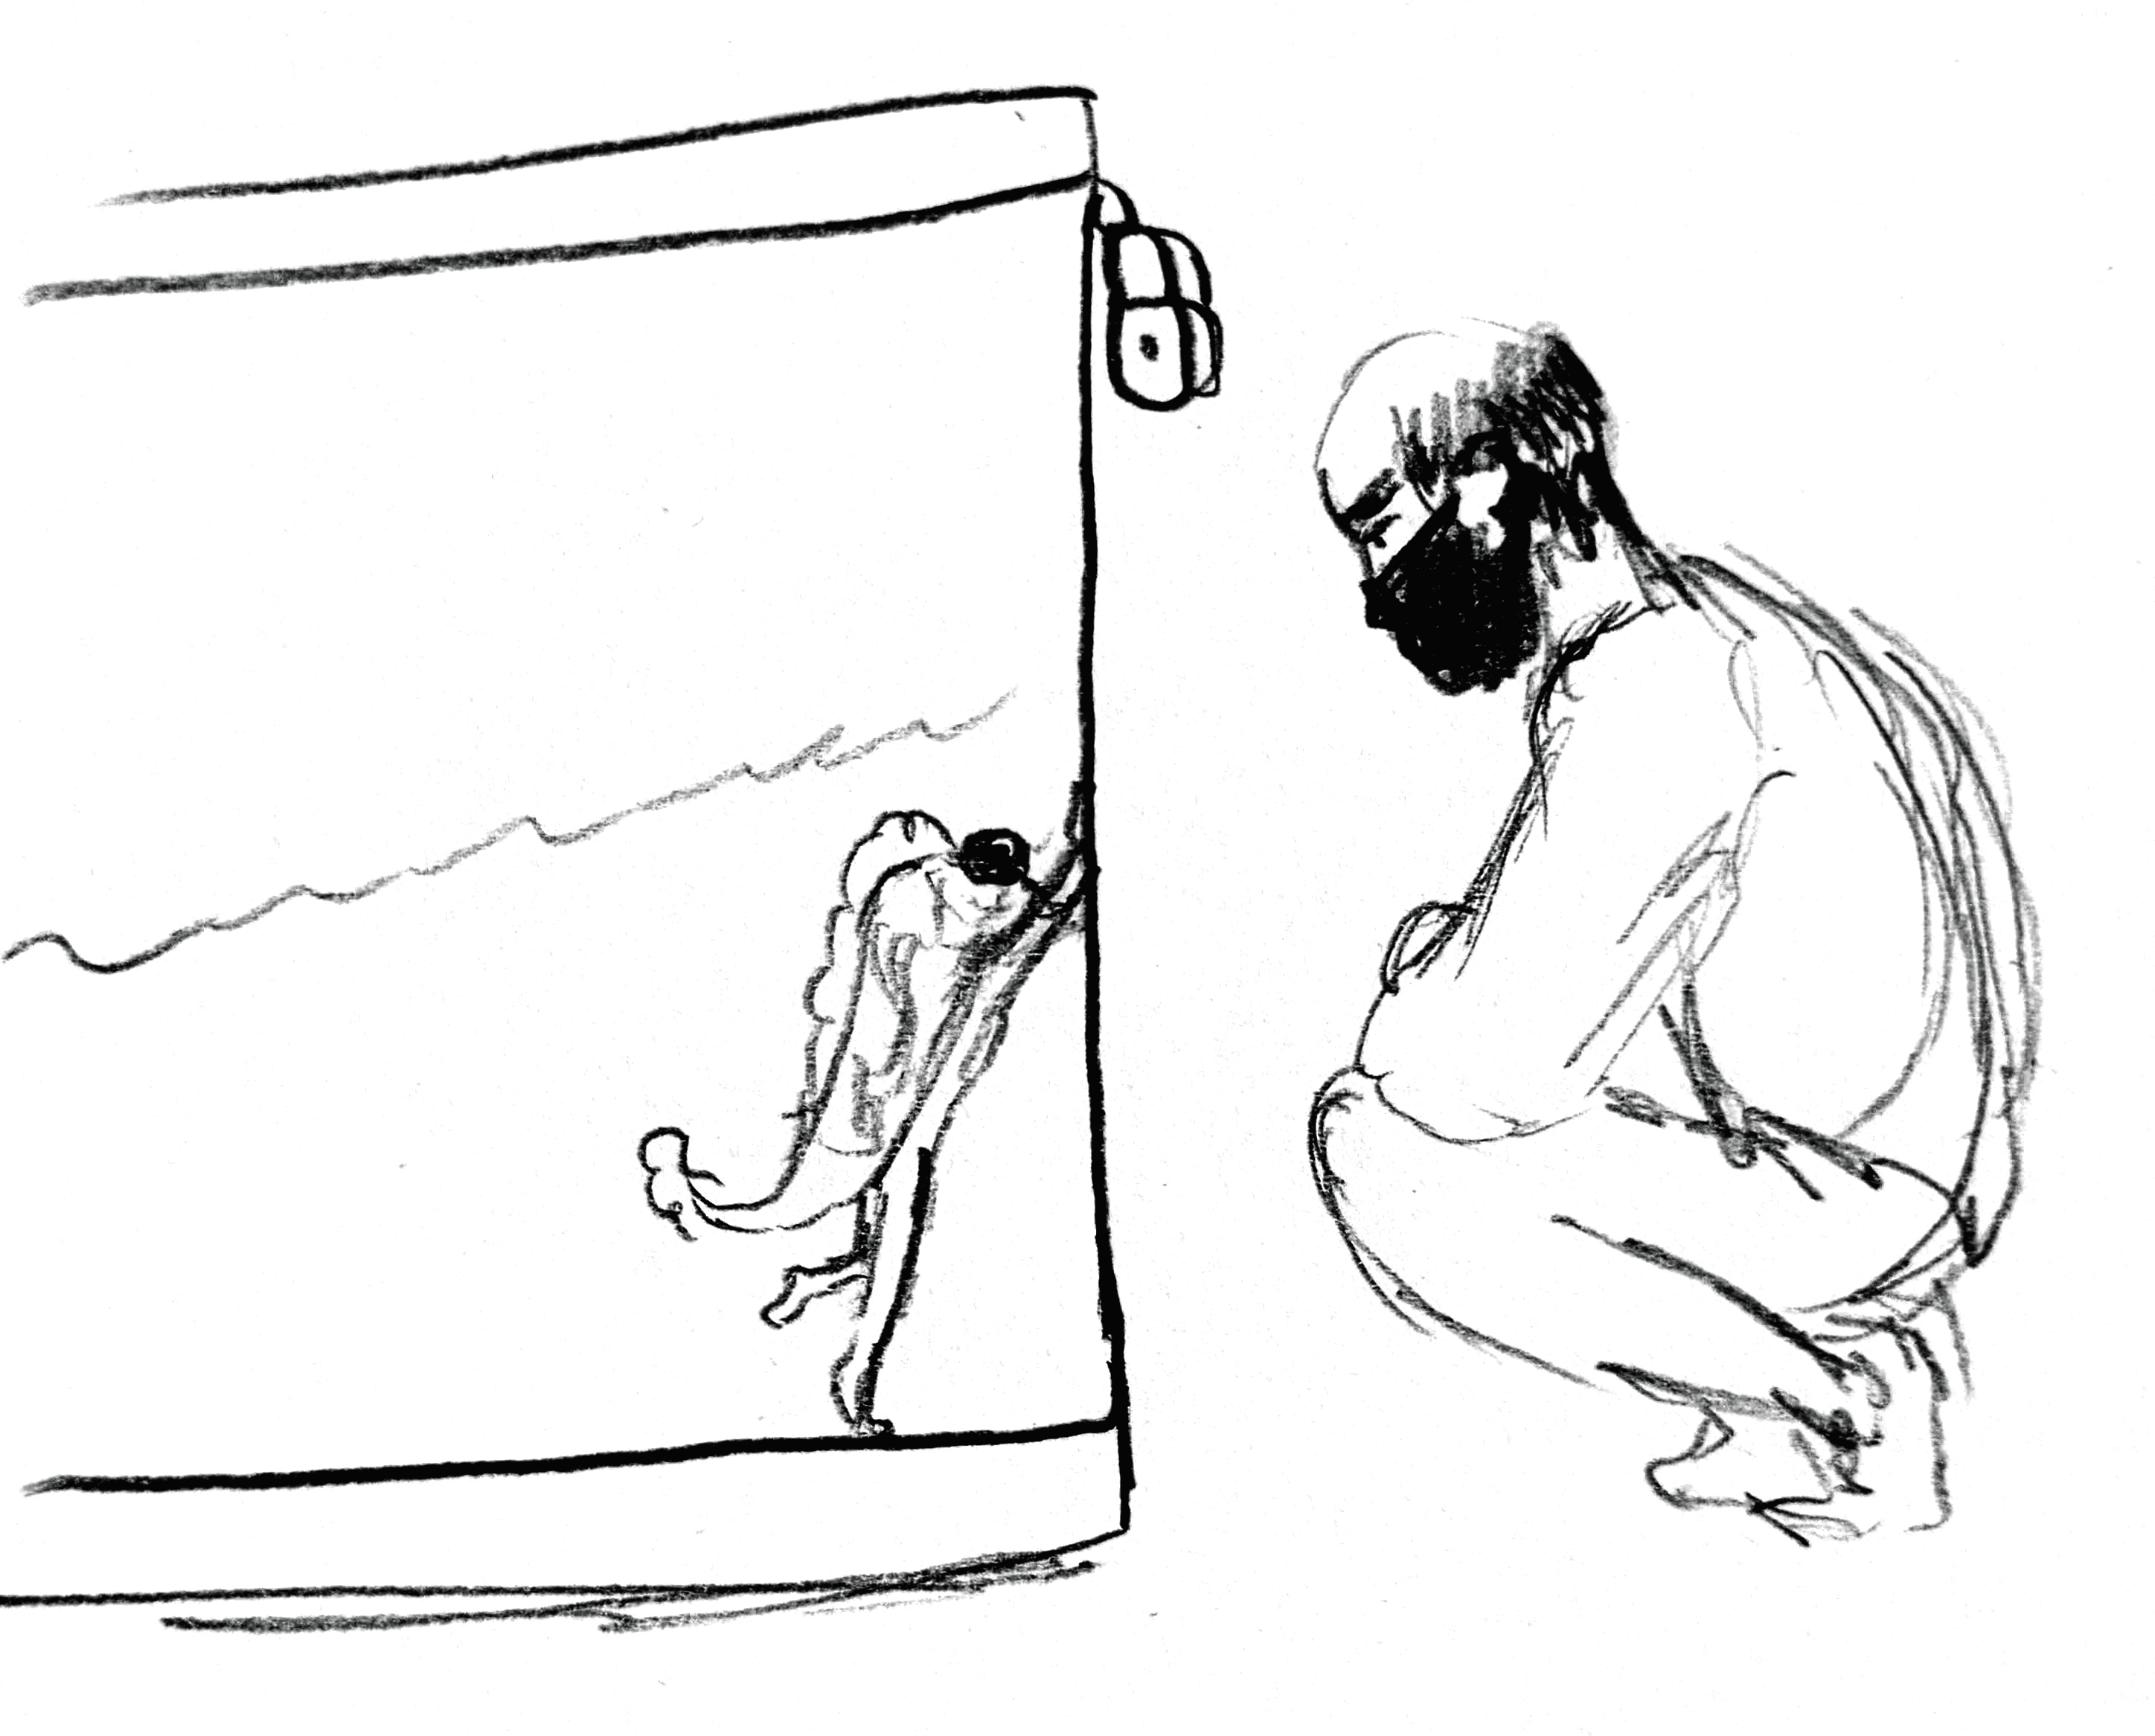
\includegraphics[width=0.5\textwidth]{3}
\end{center}

El niño le dijo que se llamaba Carles. Le dijo que quería ser un pescador cuando fuera grande. Le dijo que quería atrapar peces como Roger y llevarlos a su acuario para resguardarlos de las duras corrientes. A Roger no le gustaba. Desdeñaba la idea de que un niño como Carles creciese para convertirse en aquello me más odiaba: un encarcelador.

Carles tenía la suerte de poder visitar el zoo todos los días y siempre se detenía en la jaula de Roger para hablar con él. A Roger le gustaba Carles. Era el único amigo que tenía en este lugar.

Un día, Carles le dijo a Roger que iba a ser libre. Le dijo que iba a llevarlo a su casa y que iba a cuidar de él. Roger no podía creerlo. Al día siguiente, Carles empezó la misión de rescate. Ambos sabían que no iba a ser fácil. Tuvo que entrar a través del la entrada del personal. Pasar desapercibido no fue tan difícil ya que Carles llevaba un chaleco verde reflectante y una escalera. La triste cara de Roger cambió en el instante en el que vio a Carles llegar.

Al final, Carles metió a Roger en una pequeña pecera y se lo llevó a casa. Aquí Roger tuvo el lujo de tener una gran casa, una casa con una enorme piscina y una fuente de agua. Había comida fresca y limpia, y un equipo de música para bailar. Incluso había un televisor para ver y un ordenador para jugar.

Durante el primer día, Roger estuvo tan feliz que no pudo parar de bailar. Carles le dijo que podía quedarse en su casa para siempre. Y Roger sabía que era verdad. Tenía una familia nueva y un hogar al que pertenecer. Finalmente, era libre.  Pero su sueño de nadar a contracorriente lo mantenía inquieto. Los ríos de Europa eran su casa, no una piscina y un equipo de música.

Antes de irse, Roger tenía que parar a Carles; no podía dejar que este fuera un pescador. Para lograrlo, Roger sabía que tendría que enseñarle a Carles lo mal que lo pasaban los peces al ser atrapados. Por eso llevó a Carles a un río, y este pudo ver por sí mismo lo duro que era la vida para los salmonetes. Carles lloró al ver lo mal que lo pasaban los peces y juró que nunca más iba a pescar.

A pesar de que Roger se había marchado, ambos siguieron siendo amigos y pasaron los siguientes años ayudando a los peces del río. Roger lloraba, pero esta vez no de tristeza, sino de alegría.


\vspace*{\fill}
\begin{center}
    
\includegraphics[width=1\textwidth]{4}
\end{center}

\end{document}